



\section{Results and Discussion}

%We measure the performance of proofreading quantitatively by comparing VI scores of segmentations against ground truth labelings. Lower VI scores indicate less distance to the ground truth and a better segmentation. For all experiments, we report the VI score of the initial segmentation followed by the VI score of the proofreading output.

\subsection{Precision and Recall}

We compare the guided proofreading and focused proofreading classifiers and report precision and recall as well as f1 scores across datasets.

\paragraph{L. Cylinder.} Evaluation was performed on previously unseen sections of mouse cortex volume of Kasthuri~\etal~\cite{kasthuri2015saturated}. We generated an unbalanced dataset of 81,184 correct and 8,780 split error patches in respect to the ground truth labeling. We then ranked each patch by using focused proofreading, guided proofreading and compared precision/recall (Table \ref{tab:prcyl}. Our method exhibits higher precision and recall for correct and error patches.

\begin{table}[h]
\caption{Classifier comparison on an unbalanced test set of the L. Cylinder volume.}%While the training of our classifier is more expensive, testing accuracy is superior. }

\small{
\begin{tabular}{l|c|c|c|c}

 & precision & recall & f1 score & \# \\ 
\textbf{Focused Proofreading} & ~ & ~ & ~ & ~ \\ 
correct & 0.93 & 0.31 & 0.47 & 81,184 \\ 
split error & 0.11 & 0.78 & 0.19 & 8,780 \\ 
\textbf{Guided Proofreading} & ~ & ~ & ~ & ~ \\ 
correct & 1.00 & 0.93 & 0.96 & 81,184 \\ 
split error & 0.61 & 0.96 & 0.74 & 8,780 \\ 
\end{tabular} 
}
\label{tab:prcyl}
\end{table}

\paragraph{AC4 subvolume.} We generated 3,488 correct and 332 error patches (10 merge errors, 322 split errors). Again, guided proofreading achieves better precision/recall scores (Table \ref{tab:prac4}).

\begin{table}[h]
\caption{Classifier comparison on correct and split error patches of the AC4 subvolume.}%While the training of our classifier is more expensive, testing accuracy is superior. }

\small{
\begin{tabular}{l|c|c|c|c}

 & precision & recall & f1 score & \# \\ 
\textbf{Focused Proofreading} & ~ & ~ & ~ & ~ \\ 
correct & 0.94 & 0.69 & 0.80 & 3,488 \\ 
split error & 0.14 & 0.51 & 0.21 & 332 \\ 
\textbf{Guided Proofreading} & ~ & ~ & ~ & ~ \\ 
correct & 1.00 & 0.92 & 0.96 & 3,488 \\ 
split error & 0.54 & 0.95 & 0.69 & 332 \\ 
\end{tabular} 
}
\label{tab:prac4}
\end{table}

\subsection{Forced Choice User Experiment}
We performed a user study to evaluate the forced choice error correction method among novices and experts. To be comparable to Haehn's~\etal Dojo user study, participants were asked to proofread the AC4 subvolume for 30 minutes. We counted 10 merge errors and 322 split errors by computing the maximum overlap of the initial segmentation with respect to the ground truth labeling (both provided by Haehn~\etal). For evaluation, we measure the performance of proofreading quantitatively by comparing VI scores of segmentations relative to ground truth. The median VI of the initial segmentation was $0.476$ ($SD=0.089$), mean VI was $0.512$ ($SD=0.09$). Most novices and all experts were able to improve upon this score with both, focused proofreading and guided proofreading (Fig.~\ref{fig:ac4trails}).

\paragraph{Novice performance.} Participants using focused proofreading were able to reduce the median VI of the automatic segmentation to $0.469$ ($SD=0.87$). On average, users viewed $423.4$ corrections and accepted $45.8$ of them with an average time of $4.9$ seconds spent per correction. Participants using guided proofreading were able to reduce the median VI to $0.424$ ($SD=0.037$). Here, users viewed on average $353.4$ corrections and accepted $106.9$ in $6.2$ seconds. While three users of focused proofreading made the initial segmentation worse, all participants using guided proofreading were able to improve it. In comparison to the results of Haehn~\etal, focused and guided proofreading outperform interactive proofreading with Dojo (median VI $0.535$, $SD=0.055$). The slope of VI score per correction in Fig.~\ref{fig:ac4trails} shows that guided proofreading enables improvements with fewer corrections than the other tools. Interestingly, novice performance decreases after approximately $300$ corrections. There are two explanations for this: user fatigue and increasing uncertainty during error suggestion from the classifier. Regarding fatigue, we suggest that future experiments include short breaks after every ten minutes.

\paragraph{Expert performance.} Domain experts were able to improve the initial segmentation in all cases. With focused proofreading, the median VI of the automatic segmentation was $0.439$ ($SD=0.084$). With guided proofreading, the median VI was $0.396$ ($SD=0.032$) as shown in Fig.~\ref{fig:ac4boxplot}.

\paragraph{Subjective responses.} All subjective responses were recorded using the NASA-TLX workload index. Mental, physical, and temporal demands were reported slightly higher for participants using focused proofreading. However, these differences were not statistically significant. This is not surprising since the user interface was the same for both control groups.

\begin{figure}[t]
\begin{center}
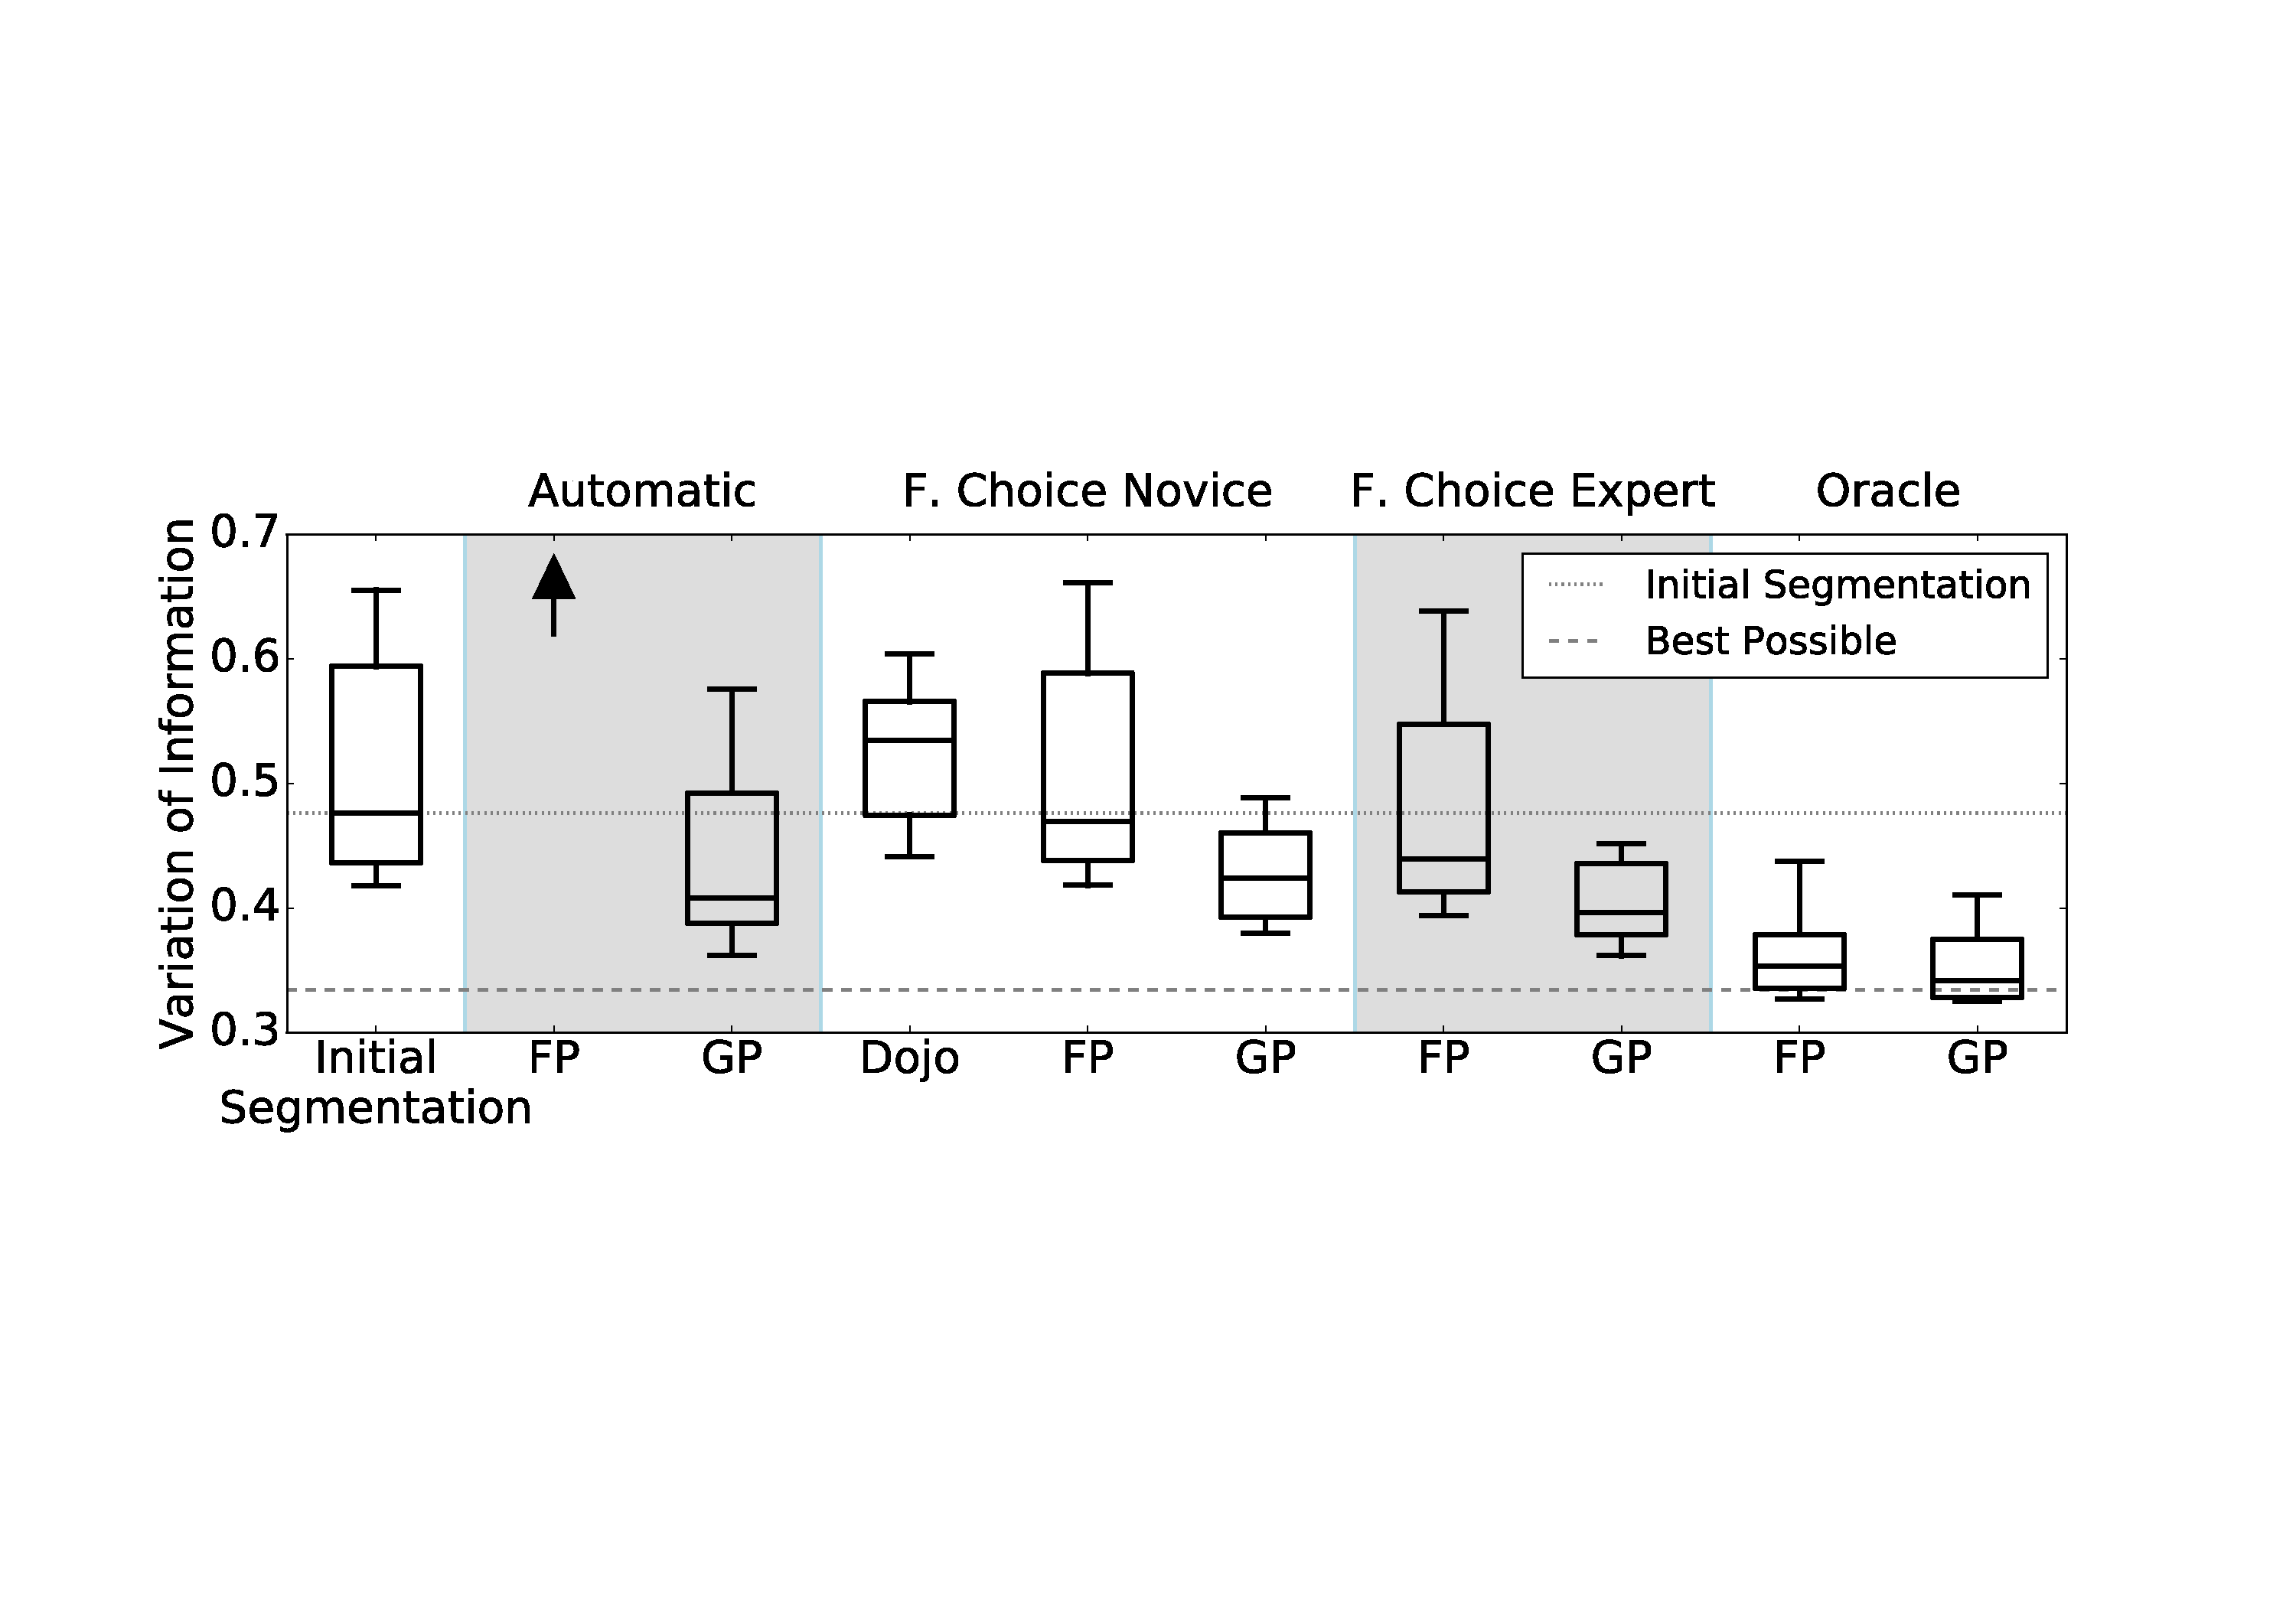
\includegraphics[width=\linewidth]{gfx/ac4boxplot.pdf}
\end{center}
  \vspace{-4mm}
   \caption{VI distributions of guided proofreading (GP), focused proofreading (FP) and Dojo output across the AC4 subvolume with different error correction approaches. The variation resulting from performance of focused proofreading with automatic selection is an order of magnitude higher (as indicated by the arrow) and is reported in the text.}
\label{fig:ac4boxplot}
\end{figure}
\subsection{Automatic Error Correction}

\paragraph{Selection oracle.} Accepting and rejecting proofreading corrections with the selection oracle yields the best performance on all datasets because all detected merge and split errors are corrected as long as the segmentation is improved. Fig.~\ref{fig:ac4trails} shows slope of VI reduction using the selection oracle on the AC4 subvolume (initial median VI $0.476$, $SD=0.089$). With focused proofreading, the selection oracle reaches a median VI of $0.353$ ($SD=0.037$) after $1605$ corrections. With guided proofreading, the oracle results in a median VI of $0.342$ ($SD=0.03$) after approximately $800$ corrections and then stagnates until all regions are proofread. Both results are very close to the best possible median VI of $0.334$ (calculated by computing maximum overlap with the ground truth). The slope of the trails in Fig.~\ref{fig:ac4trails} shows that guided proofreading requires fewer corrections to reach a reasonable reduction in VI. Fig.~\ref{fig:ac4boxplot} shows the VI distribution across methods.
The results on the L. Cylinder dataset (initial VI $0.379$, $SD=0.118$) are similar. Focused proofreading reduces the median VI to $0.298$ ($SD=0.075$) after $26,170$ corrections ($2,419$ accepted). Guided proofreading reduces the median VI to $0.2996$ ($SD=0.073$) after $27,491$ corrections ($2,696$ accepted).

\paragraph{Automatic selection with threshold.} Focused proofreading was not designed to run automatically. This explains very poor performance on the AC4 subvolume (VI of $1.9$, $SD=0.496$) and on the L. Cylinder dataset (VI of $2.75$, $SD=0.789$). For guided proofreading we define the threshold $p_t=0.95$ for both datasets. This reduces median VI in the AC4 subvolume to $0.398$ ($SD=0.068$). This is an impressive result and comparable to expert performance. Guided proofreading also reduces VI in the L. Cylinder data to $0.352$ ($SD=0.087$).

\paragraph{Merge Error Detection} Guided proofreading performs merge error detection prior to split error detection. The classifier found 10 merge errors in the AC4 subvolume of which 4 reduce VI. Automatic selection with $p_t=0.95$ corrected 6 of these errors (Prec./Recall 0.87/0.80, f1-score 0.80). This was not captured in median VI but resulted in a mean VI reduction from $0.512$ ($SD=0.09$) to $0.509$ ($SD=0.086$). The selection oracle reduced mean VI with only merge errors to $0.508$ ($SD=0.086$). In the forced choice user study, participants marked 1.9 merge errors (experts: 2) merge errors for correction and reduce mean VI to $0.502$ (experts: VI $0.503$, $SD=0.086$). This shows how hard it is to identify merge errors and how little they effect VI. In 50 sections of the L. Cylinder dataset 151 merge errors were automatically found of which 17 reduce VI. Automatic selection with $p_t=0.95$ corrected 6 true VI-reducing errors and 30 VI-increasing ones (Prec./Recall 0.82/0.73, f1-score 0.77) without - in sum - any effect on the VI. 

\subsection{Limitations}
Guided proofreading works on 2D image sections. This enables error correction without a computationally expensive alignment process. However, the output requires an additional (block-)merging step prior to 3D  analysis.
